\documentclass{article}
\usepackage[UTF8]{ctex}
\usepackage{amsmath,mathtools,geometry,pgfplots,float,mathrsfs,caption,enumerate}
\pgfplotsset{compat=1.15}
\usetikzlibrary{arrows}
\geometry{scale=0.7}

\newcommand\cusong[1]{
	\noindent \rlap{\hspace{0.01em}#1}\rlap{\hspace{0.02em}#1}\rlap{\hspace{0.03em}#1}\rlap{\hspace{0.04em}#1}\rlap{\hspace{0.05em}#1}#1
}

\title{\cusong{每日一题(20.1)}}
\author{\kaishu 门宇翎}
\date{2022年6月7日}

\begin{document}
\maketitle
\begin{enumerate}
	\renewcommand{\labelenumi}{\textbf{\theenumi. }}
	\item 在$\triangle ABC$中, $\angle BAC=5.25^\circ$, $AD$为$\angle BAC$的平分线, 过$A$做$DA$的垂线交直线$BC$于$M$. 若$BM=BA+AC$, 试求$\angle ABC$与$\angle ACB$的度数. (\kaishu 1991年北京市初中竞赛题)
	\begin{figure}[H]
		\flushright
		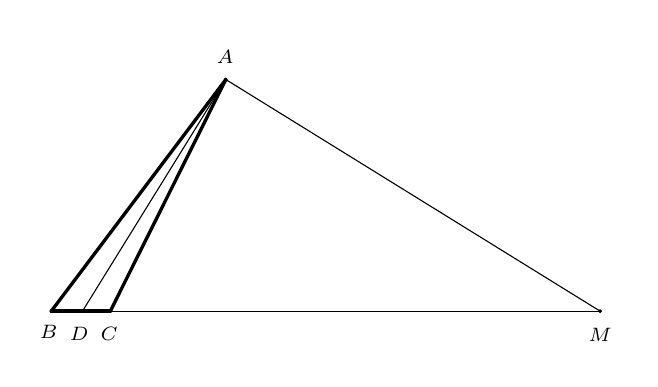
\begin{tikzpicture}[line cap=round,line join=round,>=triangle 45,x=1.5cm,y=1.5cm]
			\clip(-0.2,-0.4) rectangle (4.9,2.4);
			\draw [line width=1.2pt] (0.,0.)-- (1.4777166584145698,1.9609962393504927);
			\draw [line width=1.2pt] (1.4777166584145698,1.9609962393504927)-- (0.5,0.);
			\draw [line width=0.4pt] (0.26421536441570687,0.)-- (1.4777166584145698,1.9609962393504927);
			\draw [line width=0.4pt] (1.4777166584145698,1.9609962393504927)-- (4.646651269167756,0.);
			\draw [line width=1.2pt] (0.,0.)-- (0.5,0.);
			\draw [line width=0.4pt] (0.5,0.)-- (4.646651269167756,0.);
			\begin{scriptsize}
				\draw [fill=black] (0.,0.) circle (0.5pt);
				\draw[color=black] (-0.02142375616988858,-0.1781923314021496) node {$B$};
				\draw [fill=black] (0.5,0.) circle (0.5pt);
				\draw[color=black] (0.4898219808648679,-0.19152917671362485) node {$C$};
				\draw [fill=black] (1.4777166584145698,1.9609962393504927) circle (0.5pt);
				\draw[color=black] (1.47230291899253,2.155755598106019) node {$A$};
				\draw [fill=black] (4.646651269167756,0.) circle (0.5pt);
				\draw[color=black] (4.646472103712671,-0.20042040692127502) node {$M$};
				\draw [fill=black] (0.26421536441570687,0.) circle (0.5pt);
				\draw[color=black] (0.23642191989981468,-0.19597479181744995) node {$D$};
			\end{scriptsize}
		\end{tikzpicture}
	\end{figure}
	\item\songti 在$\triangle ABC$中, $D$为$AB$中点, 分别延长$CA$, $CB$至$E$, $F$, 使$DE=DF$. 过$E$, $F$分别作直线$CA$, $CB$的垂线, 相交于$P$. 设$PA$, $PB$的中点为$M$, $N$. 求证:
	\begin{enumerate}[(1) ]
		\item $\triangle DEM\cong\triangle FDN$; 
		\item $\angle PAE=\angle PBF$.
	\end{enumerate}
	\begin{figure}[H]
		\flushright
		\vspace*{-2cm}
		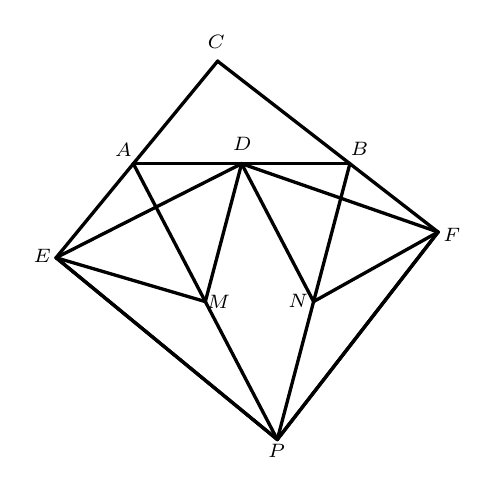
\begin{tikzpicture}[line cap=round,line join=round,>=triangle 45,x=0.55cm,y=0.55cm]
			\clip(-0.7,-0.7) rectangle (9.5,9.5);
			\draw [line width=1.2pt] (1.7402705774643774,6.359049303713263)-- (6.740270577464377,6.359049303713263);
			\draw [line width=1.2pt] (6.740270577464377,6.359049303713263)-- (3.685641923910132,8.726372764470627);
			\draw [line width=1.2pt] (3.685641923910132,8.726372764470627)-- (1.7402705774643774,6.359049303713263);
			\draw [line width=1.2pt] (8.776638884700095,4.780873029208456)-- (4.240270577464377,6.359049303713263);
			\draw [line width=1.2pt] (4.240270577464377,6.359049303713263)-- (-0.04398897131208335,4.187782878094279);
			\draw [line width=1.2pt] (-0.04398897131208335,4.187782878094279)-- (5.063952301135283,-0.00971812059380782);
			\draw [line width=1.2pt] (5.063952301135283,-0.00971812059380782)-- (8.776638884700095,4.780873029208456);
			\draw [line width=1.2pt] (1.7402705774643774,6.359049303713263)-- (5.063952301135283,-0.00971812059380782);
			\draw [line width=1.2pt] (5.063952301135283,-0.00971812059380782)-- (6.740270577464377,6.359049303713263);
			\draw [line width=1.2pt] (-0.04398897131208335,4.187782878094279)-- (3.4021114392998304,3.1746655915597275);
			\draw [line width=1.2pt] (3.4021114392998304,3.1746655915597275)-- (4.240270577464377,6.359049303713263);
			\draw [line width=1.2pt] (4.240270577464377,6.359049303713263)-- (5.90211143929983,3.1746655915597275);
			\draw [line width=1.2pt] (5.90211143929983,3.1746655915597275)-- (8.776638884700095,4.780873029208456);
			\draw [line width=1.2pt] (8.776638884700095,4.780873029208456)-- (5.063952301135283,-0.00971812059380782);
			\draw [line width=1.2pt] (5.063952301135283,-0.00971812059380782)-- (-0.04398897131208335,4.187782878094279);
			\draw [line width=1.2pt] (1.7402705774643774,6.359049303713263)-- (-0.04398897131208335,4.187782878094279);
			\draw [line width=1.2pt] (6.740270577464377,6.359049303713263)-- (8.776638884700095,4.780873029208456);
			\begin{scriptsize}
				\draw [fill=black] (1.7402705774643774,6.359049303713263) circle (0.5pt);
				\draw[color=black] (1.5095498712516606,6.679673472369655) node {$A$};
				\draw [fill=black] (6.740270577464377,6.359049303713263) circle (0.5pt);
				\draw[color=black] (6.958279426243702,6.692085157002869) node {$B$};
				\draw [fill=black] (3.685641923910132,8.726372764470627) circle (0.5pt);
				\draw[color=black] (3.6567713131961326,9.174422083645657) node {$C$};
				\draw [fill=black] (4.240270577464377,6.359049303713263) circle (0.5pt);
				\draw[color=black] (4.252532175700956,6.816202003335008) node {$D$};
				\draw [fill=black] (-0.04398897131208335,4.187782878094279) circle (0.5pt);
				\draw[color=black] (-0.36461450871143364,4.2345715996265065) node {$E$};
				\draw [fill=black] (8.776638884700095,4.780873029208456) circle (0.5pt);
				\draw[color=black] (9.093089183552657,4.718627300321851) node {$F$};
				\draw [fill=black] (5.063952301135283,-0.00971812059380782) circle (0.5pt);
				\draw[color=black] (5.046879992374056,-0.2832816068633709) node {$P$};
				\draw [fill=black] (3.4021114392998304,3.1746655915597275) circle (0.5pt);
				\draw[color=black] (3.7064180517382015,3.1795784058033205) node {$M$};
				\draw [fill=black] (5.90211143929983,3.1746655915597275) circle (0.5pt);
				\draw[color=black] (5.543347377794744,3.191990090436535) node {$N$};
			\end{scriptsize}
		\end{tikzpicture}
	\end{figure}
	\rightline{\kaishu(2003年全国初中联赛题)}
\end{enumerate}
\end{document}